% !TeX document-id = {2fa47047-5258-46cc-82b6-1018c6ae19b3}
\documentclass[8pt, table, aspectratio=169]{beamer}
\usetheme{Warsaw}
%\usecolortheme{lily}

% !TeX TXS-program:compile = txs:///pdflatex/[--shell-escape]

\usepackage{amsmath,amssymb,amsfonts,amsthm}
\usepackage{animate}
\usepackage{graphicx}
\usepackage{epsfig,epstopdf}
\usepackage{verbatim}
\usepackage{subfig}
\usepackage{textpos}
\usepackage{beamertexpower}
\usepackage{multirow}
\usepackage{booktabs}
\usepackage{tikz}
\usepackage{pgfplots}
\usepackage{bm}
\usepackage{etoolbox}
\usepackage{caption}
\usepackage{natbib}
\usepackage{xcolor}
\usepackage{tikz}
\usepackage{mathtools}
\usepackage{minted}
\usepackage{multimedia}

\usetikzlibrary{calc,shapes}
\usetikzlibrary{arrows,shapes}
\usetikzlibrary{calc,3d}

% for the code snippets

\usepackage{scrextend}

\addtokomafont{labelinglabel}{\sffamily}
\definecolor{grey}{rgb}{0.8,0.8,0.8}
\definecolor{lightgrey}{rgb}{0.9,0.9,0.9}
\usetikzlibrary{arrows,shapes}

\definecolor{CASgray}{RGB}{176,174,175}
\definecolor{CASblue}{RGB}{50,70,123}
\definecolor{CASred}{RGB}{227,33,36}
\definecolor{CASgreen}{RGB}{153,153,102}
\definecolor{CASblack}{RGB}{35,31,32}
\definecolor{CASbackground}{RGB}{250,250,250}

\setbeamercolor{block title}{bg=CASblue,fg=white}
\setbeamercolor{block title alerted}{bg=CASred,fg=white}
\setbeamercolor{block title example}{bg=CASgreen,fg=white}

\usefonttheme{professionalfonts}

\setbeamertemplate{navigation symbols}{}
\setbeamertemplate{itemize items}[triangle]
\setbeamertemplate{enumerate items}[default]

\setbeamercolor{item projected}{bg=CASblack}
\usesubitemizeitemtemplate{%
	\tiny\raise1.5pt\hbox{\color{CASblack}$\blacktriangleright$}%
}

% Remove the default footer content
\setbeamertemplate{footline}{}

% Remove the default header content
\setbeamertemplate{headline}{}

% Set frametitle text to black and remove both the background and gradient
\setbeamercolor{frametitle}{fg=black, bg=}  % Set background to white for transparency
\setbeamerfont{frametitle}{size=\Large} 

% Optionally, you can remove the border as well
\setbeamertemplate{frametitle}[default][left]  % Reset any custom frametitle templates


% Remove the blue band by setting the header background to transparent
\setbeamercolor{headline}{bg=}

% Set text color to black
\setbeamercolor{normal text}{fg=black}

\addtobeamertemplate{background}{
	\begin{tikzpicture}[overlay, remember picture]
		
		% Logo in top-right
		\node[anchor=north east, xshift=-0.5cm, yshift=-0.5cm] at (current page.north east) {
			
\includegraphics[height=1cm]{figures/UTS_logo.png}
		};
		
		% Transparent black footer rectangle
		\fill[black, opacity=0.20] 
		(current page.south west) rectangle 
		([yshift=0.7cm]current page.south east);
		
		% Bottom-left "UTS" text
		\node[anchor=south west, xshift=0.5cm, yshift=0.1cm, text=white, font=\bfseries\Large]
		at (current page.south west) {UTS};
		
		% Bottom-right slide number
		\node[anchor=south east, xshift=-0.5cm, yshift=0.1cm, text=white, font=\bfseries\Large]
		at (current page.south east) {\insertframenumber{}};
	\end{tikzpicture}
}{}

% Define your white footer text command
\newcommand{\customfootertext}[1]{%
	\begin{tikzpicture}[overlay, remember picture]
		\node[anchor=south west, xshift=1.5cm, yshift=0.025cm, text=white, font=\bfseries]
		at (current page.south west) {{\Large$|$} #1};
	\end{tikzpicture}%
}


\begin{document}
\pgfplotsset{compat=1.14}
%\tikzstyle{every picture}+=[remember picture,overlay]
%\tikzstyle{every picture}+=[remember picture]

\section{Introduction slide}
% Introduction slide
{
	\setbeamertemplate{footline}{} 
	\setbeamertemplate{background} 
	{
		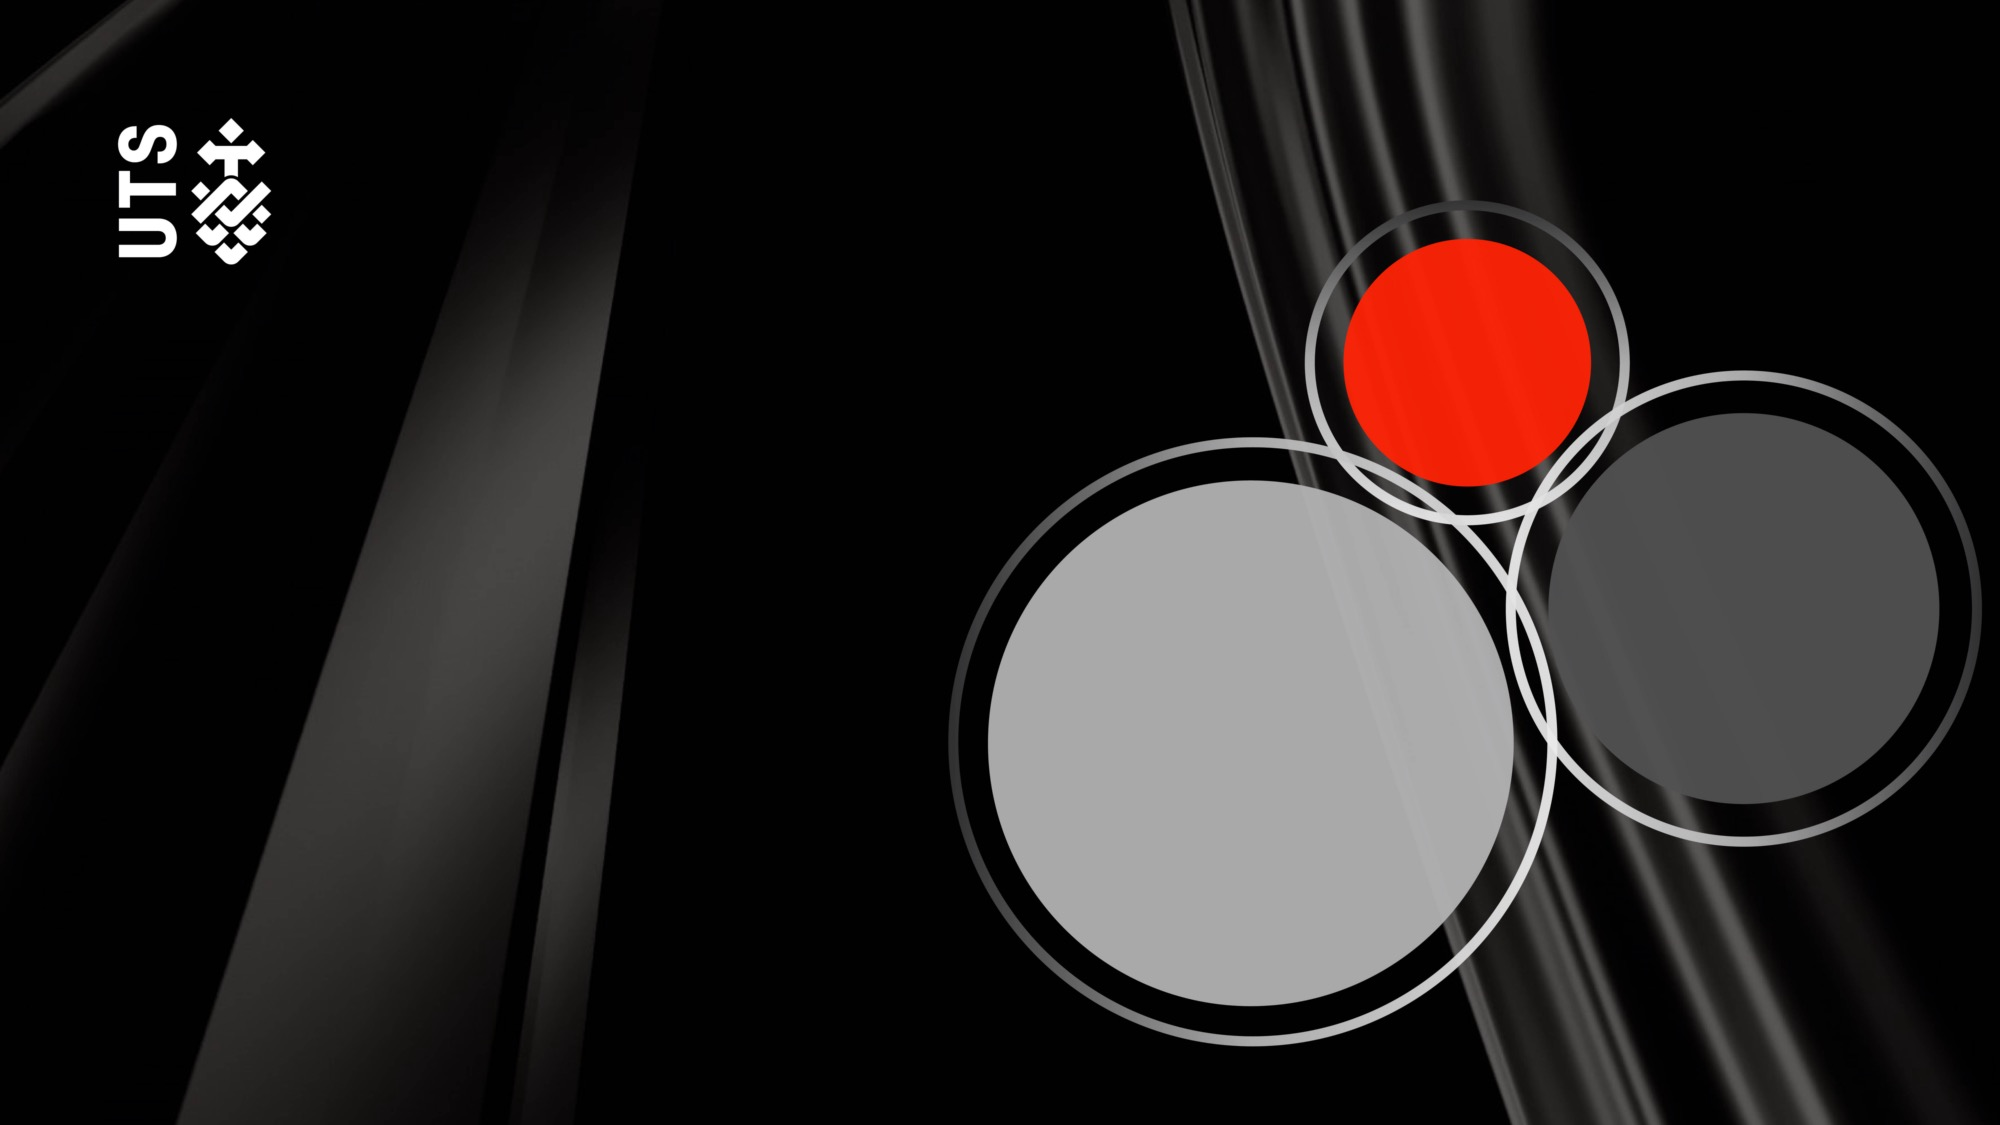
\includegraphics[width=\paperwidth,height=\paperheight]{figures/background_first_slide.jpg}
	}
	\begin{frame}
		\begin{tikzpicture}[overlay, remember picture]
			\node[anchor=west, text=white, font=\Huge\bfseries] at (1.5,1.9) {Robotics Institute};
			\node[anchor=west, text=white, font=\huge\bfseries] at (0.0,0) {Course};
			\node[anchor=west, text=white, font=\huge\bfseries] at (0.0,-1) {Title};
			\node[anchor=west, text=white, font=\huge\bfseries] at (0.0,-2) {Author};
		\end{tikzpicture}
	\end{frame}
}

\section{Introduction}

%%%%%%%%%%%%%%%%%%%%%%%%%%%%%%%%%%%%%%%%%%%%%%%%%%%%%%%%%%%%%%%%%%%%%%%%%%%%%%%%%%%%%%%%%%%
% CNN introduction
\begin{frame}{CNNs: inspiration}
	\begin{columns}[T] % align columns
		\begin{column}{.5\textwidth}
			Cat's visual cortex is made of neurons [{\color{blue}\href{http://onlinelibrary.wiley.com/doi/10.1113/jphysiol.1962.sp006837/pdf}{Hubel 1962}}]:
			\begin{figure}
				\centering
				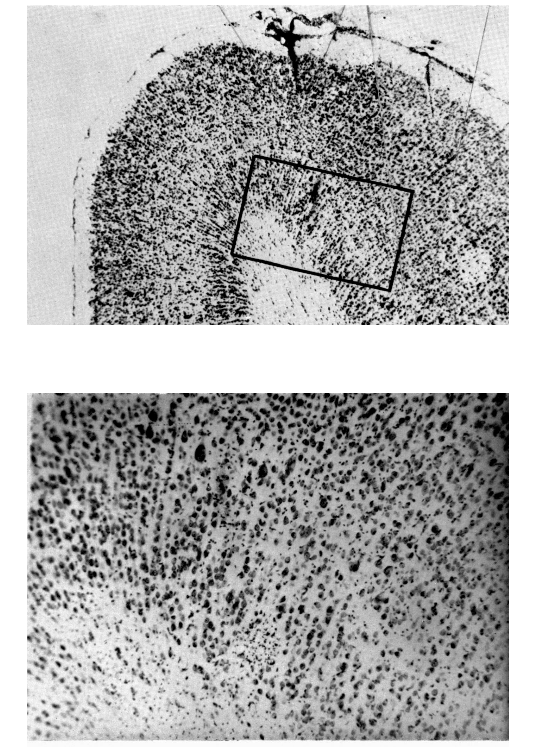
\includegraphics[width=0.65\linewidth]{figures/cat_visual_cortex_neurons.png}
			\end{figure}
		\end{column}%
		%\hfill%
		\begin{column}{.35\textwidth}
			Convoluted Neural Networks (CNNs)
			{\color{blue}\rule{\linewidth}{4pt}}
			What is it?
			\begin{itemize}
				\item[$\bullet$] Supervised algorithm
				\item[]
				\item[$\bullet$] Based on Neural Networks
				\item[]
				\item[$\bullet$] Embed the feature engineering
				\item[]
			\end{itemize}
			Replace some of the hidden layers by
			\begin{itemize}
				\item[$\bullet$] Convolution layers
				\item[$\bullet$] Max pooling layers
				\item[$\bullet$] ReLU layers
				\item[$\bullet$] Fully-connected layers
			\end{itemize}
		\end{column}%
	\end{columns}
	
\end{frame}

\section{Convolutional Neural Networks}

%%%%%%%%%%%%%%%%%%%%%%%%%%%%%%%%%%%%%%%%%%%%%%%%%%%%%%%%%%%%%%%%%%%%%%%%%%%%%%%%%%%%%%%%%%%
\begin{frame}{CNNs: layers = convolution}
	Convolution in image processing:
    \begin{figure}
		\centering
		\animategraphics[loop,controls,autoplay,width=0.6\linewidth]{1}{figures/conv/convolution-}{0}{8}
	\end{figure}
\end{frame}




\begin{frame}{CNNs: VGG breakdown}
	VGG architecture:
	\begin{figure}
		\centering
		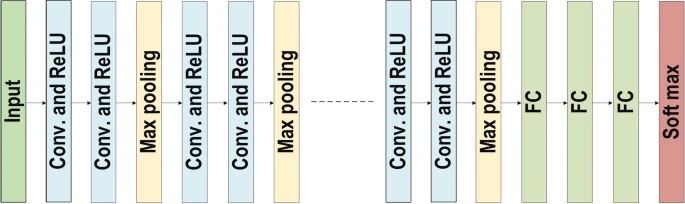
\includegraphics[width=0.8\linewidth]{figures/VGG.png}
	\end{figure}
	See the breakdown from {\color{blue}\href{http://cs231n.github.io/convolutional-networks/\#conv}{Stanford course}}.
	
	\customfootertext{\href{https://arxiv.org/pdf/1409.1556}{\emph{``Very Deep Convolutional Networks for Large-Scale Image Recognition''}, ICLR 2015}}
\end{frame}

\begin{frame}[fragile]{CNNs: implementation}
	How do you code this within Pytorch?
	\begin{exampleblock}{Python}
		\begin{overprint}
			\begin{minted}[highlightlines={4,5,11,13},fontsize=\footnotesize]{python}
class CNN(nn.Module):
	def __init__(self):
		super(CNN, self).__init__()
		self.conv1 = nn.Conv2d(1, 16, 3, 1)
		self.conv2 = nn.Conv2d(16, 32, 3, 1)
		self.fc1 = nn.Linear(32 * 5 * 5, 128)
		self.fc2 = nn.Linear(128, 10)

	def forward(self, x):
		# feature encoder
		x = F.relu(self.conv1(x))   # Layer 1
		x = F.max_pool2d(x, 2, 2)
		x = F.relu(self.conv2(x))   # Layer 2
		x = F.max_pool2d(x, 2, 2)
		
		# classifier
		x = x.view(-1, 32 * 5 * 5)
		x = F.relu(self.fc1(x))     # Fully connected layer
		x = self.fc2(x)
		return x
		\end{minted}
		\end{overprint}
	\end{exampleblock}
\end{frame}


\begin{frame}{movie}
	\begin{figure}[h!]
		\centering    
		\movie[label=show3,width=0.7\textwidth,poster
		,autostart,showcontrols,loop] 
		{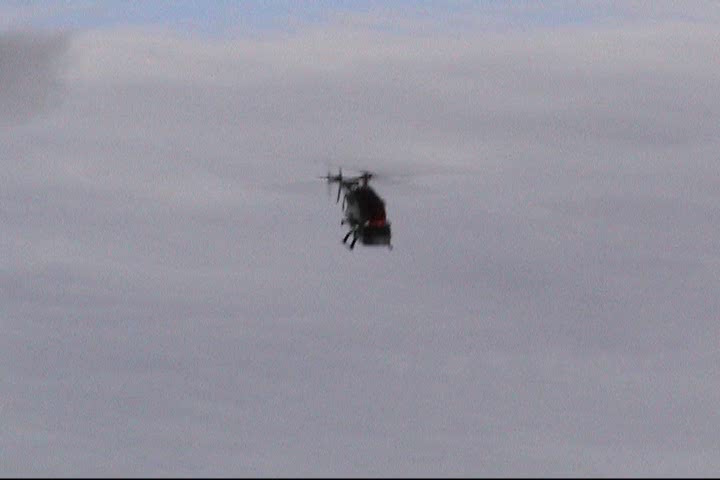
\includegraphics[width=0.7\textwidth]{figures/image26.png}}{media/media25.avi}
		\caption{caption}
	\end{figure} 
\end{frame}


\end{document}





